\documentclass[../main.tex]{subfiles}
\begin{document}
\chapter{Fundamentals of Forces}
\section{Newton's Second Law}
Once there is more than one particle in in the universe, there will be \textit{interactions} between the particles.
In Newtonian physics such interactions are described by \textit{forces}.\quad
\begin{definition}[Momentum]
  The \textit{momentum} of a point particle is the product of its \textit{mass} and its \textit{velocity}:
  \[
    \vec{p} = m \dot{\vec{x}}
  \]
  where $m$ is the \textit{inertial mass}, often shortened to just \textit{mass}.
\end{definition}
The mass is an additional property of point particles.
It could change with time, but we assume that it is constant unless otherwise specified.
\begin{law}[Newton's Second Law]
  In an inertial frame:
  \[
    \dot{\vec{p}} = \vec{F}
  \]
  That is, the rate of change of momentum is equal to the force.
  \label{newton2}
\end{law}
The force $\vec{F}$ depends on the interaction, however, we require that it must only depend on $\vec{x}$ and $\dot{\vec{x}}$.
This means that Newton's 2nd law is a second order differential equation for $\vec{x}(t)$.
Thus, given $\vec{x}$ and $\dot{\vec{x}}$ of all particles in a system at some time, Newton's equations uniquely determine $\vec{x}(t)$ for all future and past times.
The force cannot depend exclusively on time because there is no preferred time in the universe as we saw in \cref{galileanRelativity}.
\begin{remark}
  Newtonian mechanics has been superseded by both quantum mechanics (generally, small things) and relativity (generally, fast things), but nevertheless accurately describes much of the universe.
\end{remark}
\section{Conservative Forces}
\begin{definition}[Conservative Force]
  A \textit{conservative force} can be written as:
  \label{conservativeForce}
  \[
    \vec{F} = - \nabla V
  \]
  for some \textit{potential} $V$, a scalar function.
\end{definition}
\begin{remark}[Derivative Notation]\par
  From Vector Calculus, the gradient $\nabla V$ is the vector:
  \[
    \nabla V = \left(\pderiv{V}{x_1}, \pderiv{V}{x_2}, \pderiv{V}{x_3}\right)
  \]
  The notation $\partial_i f$ is often used as a shorthand for $\pderiv{f}{x_i}$.
\end{remark}
\subsection{Gravitational Potential Energy}
\label{gravity}
The \textit{gravitational potential energy} of a particle of mass $m$ at $\vec{x}$ due to a particle of mass $M$ at $\vec{x}_0$ is:
\[
  V = - \frac{GMm}{|\vec{x} - \vec{x}_0|}
\]
where $G \approx \qty{6.67e-11}{\metre^3\kilogram^{-1}\second^{-2}}$ is the \textit{gravitational constant}.

We can find $\nabla|\vec{x} - \vec{x}_0|$ by computing $\partial_i|\vec{x} - \vec{x}_0|^2$ in two ways:
\begin{align*}
  \partial_i(|\vec{x} - \vec{x}_0|^2) &= 2|\vec{x} - \vec{x}_0|\partial_i|\vec{x} - \vec{x}_0| \\
  \partial_i((\vec{x} - \vec{x}_0)_j (\vec{x} - \vec{x}_0)_j) &= 2(\vec{x} - \vec{x}_0)_j \partial_i(x_j - {x_0}_j) = 2(\vec{x} - \vec{x}_0)_j \delta_{i j} = 2(\vec{x} - \vec{x}_0)_i
\end{align*}
Combining the above yields:
\[
  2|\vec{x} - \vec{x}_0|\partial_i |\vec{x} - \vec{x}_0| = 2(\vec{x} - \vec{x}_0)_i \implies  \partial_i|\vec{x} - \vec{x}_0| = \frac{(\vec{x} - \vec{x}_0)_i}{|\vec{x} - \vec{x}_0|}
\]
Therefore:
\[
  \nabla |\vec{x} - \vec{x}_0| = \frac{\vec{x} - \vec{x}_0}{|\vec{x} - \vec{x}_0|}
\]
and so:
\[
  F = - \nabla V = -GMm \frac{\nabla|\vec{x} - \vec{x}_0|}{|\vec{x} - \vec{x}_0|^2} = -GMm \frac{\vec{x} - \vec{x}_0}{|\vec{x} - \vec{x}_0|^3}
\]
If we let $\vec{r} = \vec{x} - \vec{x}_0$ be the vector that points from $\vec{x}_0$ to $\vec{x}$ then:
\[
  F = -\frac{GMm}{r^2} \uvec{r} \text{ where } \uvec{r} = \frac{\vec{r}}{|\vec{r}|}
\]
which is the \textit{inverse square law of gravity}.
The force is going in the opposite direction to $\uvec{r}$ so the force acting on the particle of mass $m$ at $\vec{x}$ is attractive towards the particle of mass $M$ at $\vec{x}_0$, as expected.

Sometimes we write $V = m \Phi$ where $\Phi = -\frac{GM}{|\vec{x} - \vec{x}_0|}$ is called the \textit{gravitational potential}.

Near the surface of the Earth, take $\vec{x}_0 = \vec{0}$ to be the centre of the Earth and $|\vec{x}| = R + z$, where $R$ is the radius of the Earth and $z \ll R$ is the distance above the surface.
\begin{align*}
  \Phi(R + z) &= - \frac{GM}{R + z} \\
              &\approx -\frac{GM}{R}\left[1 - \frac{z}{R} + \frac{z^2}{R^2} + \cdots\right] \\
              &\approx \text{constant} + \frac{GM}{R^2} z + \cdots
\end{align*}
We define $g = \frac{GM}{R^2} \approx \qty{9.81}{\metre\second^{-2}}$ on Earth.
So $\Phi(R + z) \approx \text{constant} + gz$ near the earth.
Using this approximation, when we take the gradient, the constant drops out so $\nabla \Phi = g\uvec{z}$.
Thus $\vec{F} = -m\nabla \Phi = -mg\uvec{z}$ which is a constant downwards force.

This force leads to the simplest nontrivial example of motion due to a force.
Newton's 2nd Law (\cref{newton2}) tells us that:
\[
  m \ddot{\vec{x}} = m \vec{g} \text{ where } \vec{g} = (0, 0, -g)
\]
Considering the $z$ component:
\begin{align*}
  \cancel{m} \ddot{z} &= - \cancel{m}g \\
  \implies \dot{z} &= v_0 - gt \\
  \implies z &= z_0 + v_0 t - \frac{1}{2}gt^2
\end{align*}
where $z_0$ is the initial height and $v_0$ is the initial velocity.
\begin{remark}[Assumptions]
  \begin{itemize}
    \item We treated the Earth as a point particle, assuming that all of its mass is concentrated in a single point.
    \item We ignored non-inertial effects as technically the Earth is accelerating so is not an inertial frame.
  \end{itemize}
\end{remark}
\subsection{Energy}
\label{energySec}
\begin{definition}[Conserved Energy for Conservative Forces]
  Conservative forces have a \textit{conserved energy}:
  \begin{align*}
    E &= \frac{1}{2}m \dot{\vec{x}} \cdot \dot{\vec{x}} + V(\vec{x}) \\
      &= \frac{1}{2}m \dot{x}_i \dot{x}_i + V(\vec{x})
  \end{align*}
\end{definition}
We can check that it is constant by computing $\deriv{E}{t}$:
\begin{align*}
  \deriv{E}{t} &= m \dot{x}_i \ddot{x}_i + \pderiv{V}{x_i}\dot{x}_i \\
  &= \dot{x}_i\left(m \ddot{x}_i + \pderiv{V}{x_i}\right) \\
  &= 0 \text{ as $\vec{F} = m \ddot{\vec{x}} = -\nabla V$}
\end{align*}
\begin{example}[Escape Velocity]
  \label{escapeVelocity}
  Suppose we throw an object into space and want it to never fall back down.
  The minimal velocity the object must have to achieve this is called the \textit{escape velocity}.

  As the object is thrown:
  \[
    E_{\text{initial}} = \frac{1}{2}mv^2 - \frac{GMm}{R}
  \]
  as $V = - GMm/R$ on the surface of Earth.

  To not fall back, the object must reach $|\vec{x}| \to \infty$ without the velocity going to zero.
  Assuming that the particle reaches infinity, we have:
  \begin{align*}
    \frac{1}{2}mv^2 - \frac{GMm}{R} &= E_{\text{initial}} \\
                                    &= E_{\infty} \text{ by conservation of energy}\\
                                    &= \frac{1}{2}mv^{2}_{\infty} - 0 \text{ as $V(\vec{x}) \to 0$ as $|\vec{x}| \to \infty$}
  \end{align*}
  Since it made it to infinity, $v_{\infty}$ must be positive and thus $v^2 > 2GM/R$.
  The escape velocity is then $v_{\text{escape}} = \sqrt{2GM/R}$.
  On Earth, this is about \qty{10}{\kilo\metre\second^{-1}}.

  Note that the mass of the object $m$ cancels in $v_{\text{escape}}$ because the \textit{gravitational mass} (that appears in the inverse square law), is the same as the \textit{inertial mass} (that appears in Newton's 2nd Law -- \cref{newton2}).
  This hypothesis is known as the \textit{principal of equivalence}.
\end{example}
It is useful to write $E = T + V$ where $T = \frac{1}{2} m \dot{\vec{x}} \cdot \dot{\vec{x}}$ is the \textit{kinetic energy} and $V$ is the potential energy.

\begin{definition}[Work Done]
  The \textit{work done} by a force along a trajectory $C$ is defined to be the line integral:
  \[
    W = \int_C \vec{F} \cdot \d{\vec{x}}
  \]
\end{definition}
\begin{proposition}[Path independence of work done for conservative forces]
  Conservative forces have the property that the \textit{work done} by the force as a particle moves along a trajectory only \textbf{depends on the endpoints of the trajectory} and \textbf{not} on the path itself.
\end{proposition}
There are two ways to see this:
\begin{proof}[1]
  \begin{align*}
    W = \int_C \vec{F} \cdot \d{\vec{x}} &= \int_{t_1}^{t_2} \underbrace{\vec{F} \cdot \deriv{\vec{x}}{t}}_{\text{Power}} \d{t} \\
                                         &= m \int_{t_1}^{t_2} \ddot{\vec{x}} \cdot \dot{\vec{x}} \d{t} \text{ by Newton's 2nd} \\
                                         &= \frac{1}{2}m \int_{t_1}^{t_2} \deriv{}{t}(\dot{\vec{x}} \cdot \dot{\vec{x}}) \d{x} \\
                                         &= T(t_2) - T(t_1) \text{ as $T(t) = \frac{1}{2} m (\dot{\vec{x}}(t) \cdot \dot{\vec{x}}(t))$}\\
                                         &= V(t_1) - V(t_2) \text{ as $E_1 = V_1 + T_1 = V_2 + T_2 = E_2$}\\
                                         &= V(\vec{x}(t_1)) - V(\vec{x}(t_2)) \\
                                         &= V(\vec{x}_1) - V(\vec{x}_2)
  \end{align*}
  which only depends on the endpoints $\vec{x}_1$ and $\vec{x}_2$.

  Writing $V(t_1)$ and $V(t_2)$ is an abuse of notation as $V$ is a function of $\vec{x}$ but we write this to mean the potential at $\vec{x}(t_1)$ and $\vec{x}(t_2)$ respectively.
\end{proof}
\begin{proof}[2]
  Using the fundamental theorem of calculus for line integrals from Vector Calculus, we have:
  \begin{align*}
    T &= \int_{C} \vec{F} \cdot \d{\vec{x}} \\
      &= - \int_{C} \nabla V \cdot \d{\vec{x}} \\
      &= V(\vec{x}_1) - V(\vec{x}_2)
  \end{align*}
  which again only depends on the endpoints $\vec{x}_1$ and $\vec{x}_2$.
\end{proof}
\begin{definition}[Power]
  The \textit{power} is defined as:
  \[
    P \equiv \vec{F} \cdot \dot{\vec{x}}
  \]
  It is the rate of doing work.
\end{definition}
\section{Electromagnetic Forces}
\subsection{Lorentz Force}
\label{lorentzForce}
Forces that depend on the velocity typically do not have a conserved energy (e.g. frictional forces), however, the \textit{Lorentz force} is an exception.

\begin{definition}[Lorentz Force]
  Electromagnetic fields exert the following force on a particle with \textit{charge} $q$ at position $\vec{x}$:
  \[
    \vec{F} = q[\vec{E}(\vec{x}) + \dot{\vec{x}} \times \vec{B}(\vec{x})]
  \]
  where $\vec{E}$ is the \textit{electric field} and $\vec{B}$ is the \textit{magnetic field}.
\end{definition}
\begin{remark}[Charge]
  \textit{Charge} is another property that point particles can have.
  Unlike mass, it can be both positive or negative.
  For an electron $q \approx \qty{-1.6e-19}{\coulomb}$ which is the negative of the \textit{elementary charge} $e$.
\end{remark}
For this course, we will only consider \textit{static} electric and magnetic fields that \textbf{are independent of time}.
Static electric fields can be written in the form:
\[
  \vec{E} = -\nabla \phi(\vec{x})
\]
where $\phi$ is called the \textit{electric potential}.

\begin{proposition}[Conserved Energy in Electromagnetic Field]
  The conserved energy in an electromagnetic field is $E = \frac{1}{2} m \dot{\vec{x}} \cdot \dot{\vec{x}} + q\phi(\vec{x})$.
\end{proposition}
\begin{proof}
  We can check that it is conserved by computing $\deriv{E}{t}$:
  \begin{align*}
    \deriv{E}{t} &= m \ddot{\vec{x}} \cdot \dot{\vec{x}} + q \nabla \phi \cdot \dot{\vec{x}} \\
                 &= (\vec{F} + q\nabla\phi) \cdot \dot{\vec{x}} \text{ by Newton's 2nd} \\
                 &= (\vec{F} - q\vec{E}) \\
                 &= q(\dot{\vec{x}} \times \vec{B}) \cdot \dot{\vec{x}} \text{ using Lorentz force}\\
                 &= 0
  \end{align*}
  So $\deriv{E}{t} = 0$ and thus $E = \text{constant}$.
\end{proof}
The velocity-dependent force ($\dot{\vec{x}} \times B$) is orthogonal to the trajectory of the particle so \textbf{does no work on the particle} and thus \textbf{energy is conserved}.
This is unlike, for example, a frictional force, where the velocity-dependent force is not orthogonal to the trajectory so \textbf{work is done on the particle} and so \textbf{energy is not conserved}.

\subsection{Electric Forces}
\label{electricForces}
Electric forces are similar to gravitational forces explored in \cref{gravity}.

The potential $\phi$ at $\vec{x}$ due to another particle of charge $Q$ at $\vec{x}_0$ is:
\[
  \phi(\vec{x}) = \frac{Q}{4\pi \varepsilon_0} \frac{1}{|\vec{x} - \vec{x}_0|}
\]
where $\varepsilon_0 \approx \qty{8.85e-12}{\metre^{-3}\kilogram^{-1}\second^2\coulomb^2}$ is the \textit{permittivity of free space}.

Like gravity, this leads to an inverse square law:
\begin{align*}
  \vec{E} = -\nabla \phi &= -\frac{Q}{4\pi\varepsilon_0} \nabla\left[\frac{1}{|\vec{x} - \vec{x}_0|}\right] \\
                   &= \frac{Q}{4\pi\varepsilon_0} \frac{\vec{x} - \vec{x}_0}{|\vec{x} - \vec{x}_0|^3} \\
                   &= \frac{Q}{4\pi\varepsilon_0 r^2} \uvec{r} \text{ where $\vec{r} = \vec{x} - \vec{x}_0$}
\end{align*}
The force acting on the particle of charge $q$ at $\vec{x}$ due to the electric field is then:
\[
  \vec{F} = q\vec{E} = \frac{Qq}{4\pi\varepsilon_0 r^2} \uvec{r}
\]
This is called the \textit{Coulomb force}.

Similarly to with gravity, $\uvec{r}$ points from $\vec{x}_0$ of charge $Q$ to $\vec{x}$ of charge $q$.
There are two cases:
\begin{itemize}
  \item If $Q$ and $q$ both share the same sign, $Qq > 0$ so the force is repulsive (like charges repel).
  \item If $Q$ and $q$ have different signs, then $Qq < 0$ and so the force is attractive (opposite charges attract).
\end{itemize}

Since masses are always positive, this means that gravity generally dominates for large objects (e.g. planets), whilst electric forces tend to cancel out.

\subsection{Magnetic Forces}
Magnetic forces are very different to electric and gravitational forces.

A charged particle in a magnetic field obeys:
\[
  \vec{F} = m \ddot{\vec{x}} = q \dot{\vec{x}} \times \vec{B}
\]
This is a \textit{vector differential equation}.
The most direct way to solve is by equating the Cartesian components of both sides and then solving the system of couple differential equations.
To simplify matters, take $\vec{B}$ to be constant and assume WLOG that it is pointing in the $z$ direction, that is, $\vec{B} = (0, 0, B) = B \uvec{z}$.
\subsubsection{Solving Directly}
Equating the Cartesian components, we have:
\begin{align}
  m \ddot{x} &= q \dot{y} B \label{mag1} \\
  m \ddot{y} &= -q \dot{x} B \label{mag2} \\
  m \ddot{z} &= 0 \label{mag3}
\end{align}
First, looking at \cref{mag3}:
\[
  m \ddot{z} = 0 \implies z = z_0 + v_0 t
\]
so the particle moves with a constant velocity $v_0$ in the $z$ direction.

Differentiating \cref{mag1} and substituting in \cref{mag2}, we have:
\[
  m \dddot{x} = q \ddot{y}B = - \frac{q^2 \dot{x} B^2}{m} \implies \dddot{x} = - \left(\frac{q B}{m}\right)^2 \dot{x}
\]
We define $\omega = \frac{qB}{m}$ as the \textit{cyclotron frequency} and thus we have $\dddot{x} = -\omega^2 \dot{x}$, which is a second order equation for $\dot{x}$.
This is the differential equation for harmonic motion with angular frequency $\omega$ so:
\[
  \dot{x} = \widetilde{A}\sin(\omega t + \phi)
\]
where $\widetilde{A}$ and $\phi$ are arbitrary constants.

Integrating to obtain $x$, we have:
\[
  x = x_0 + A\cos(\omega t + \phi)
\]
It is faster to substitute back into \cref{mag1} so that we only have to integrate once to obtain $y$:
\begin{align*}
  \ddot{x} &= -A\omega^2 \cos(\omega t + \phi) \\
  \implies \dot{y} &= \frac{m}{qB} \ddot{x} = \frac{1}{\omega} (-A\omega^2 \cos(\omega t + \phi)) = -A\omega\cos(\omega t + \phi)
\end{align*}
Integrating to obtain $y$, we have:
\[
  y = y_0 - A \sin(\omega t + \phi)
\]
So the final solution is:
\[
  \vec{x}(t) = \begin{pmatrix}
  x_0 + A\cos(\omega t + \phi) \\
  y_0 - A\sin(\omega t + \phi) \\
  z_0 + v_0 t \\
  \end{pmatrix} = \vec{x}_0 +
  A \begin{pmatrix}
  \cos(\omega t + \phi) \\
  -\sin(\omega t + \phi) \\
  0 \\
  \end{pmatrix} + t \begin{pmatrix}
  0 \\
  0 \\
  v_0 \\
  \end{pmatrix}
\]
This has three parts:
\begin{enumerate}
  \item The initial position $\vec{x}_0$ (arbitrary constants $x_0, y_0, z_0$).
  \item Circular motion amplitude $A$ and angular frequency $\omega$ in the $x$-$y$ plane (arbitrary constants $A$ and $\phi$).
  \item Constant velocity $v_0$ in the $z$ direction (arbitrary constant $v_0$).
\end{enumerate}
\begin{remark}
  There are six arbitrary constants in total, which is expected for a system of three second order differential equations.
\end{remark}
This motion is known as \textit{cyclotron motion} and follows a helical trajectory.
The period of the cycle $T$ (i.e the time to complete a rotation cycle) is $T = \frac{2\pi}{\omega}$.

Changing the sign of the charge $q$ changes the sign of $A$ and so reverses the direction of the circular motion.
This means that positively charged particles will have circular motion in the opposite direction to negatively charged particles.

\subsubsection{Alternative Method to Solve}
If we let $\xi = x + iy$ and add \cref{mag1} and $i$ times \cref{mag2} we have:
\begin{align*}
  m \ddot{x} + im\ddot{y} &= qB(\dot{y} - i\dot{x}) = -iqB(\dot{x} + \dot{y}) \\
  \iff m \ddot{\xi} &= -iqB \dot{\xi}
\end{align*}
This is a first order separable differential equation for $\dot{\xi}$ with solution:
\[
  \dot{\xi} = \widetilde{C_1} e^{- i\omega t} \implies \xi = C_1 e^{- i\omega t} + C_2
\]
for $C_1, C_2 \in \C$.

We can have 4 arbitrary constants as it is a system of 2 second order differential equations so we can set $C_1 = Ae^{-i \phi}$, $C_2 = x_0 + iy_0$.
Substituting these into the solution for $\xi$ and then taking real and imaginary parts, we obtain the same solution as the first method:
\begin{align*}
  x &= x_0 + A\cos(\omega t + \phi) \\
  y &= y_0 - A\sin(\omega t + \phi)
\end{align*}
\begin{remark}
  Cyclotron motion is inherently related to complex numbers, see the ``quantum hall effect''.
\end{remark}
\section{Motion in One Dimension}
\subsection{Explicit Solution}
Often, problems in higher dimensions can be reduced to one-dimensional motion.
In 1D, Newton's 2nd law reduces to:
\[
  m \ddot{x} = F_x
\]
If $F_x$ is independent of the velocity, then it can always be written in terms of a potential, $V$ defined as:
\[
  V(x) = - \int_{x_0}^{x} F_x(x') \d{x'}
\]
where $x_0$ is an arbitrary reference point and $x'$ is a dummy variable.
If we differentiate this, using the fundamental theorem of calculus, we see that $F_x(x) = -\deriv{V}{x}$.
This is the 1D analogue of $\vec{F} = - \nabla V$.
The following energy is then conserved:
\[
  E = \frac{1}{2} m \dot{x}^2 + V(x)
\]
as we saw in \cref{energySec}.

Since $E = \text{constant}$, this gives us a first order differential equation for $x(t)$.
\[
  \dot{x} = \pm \sqrt{\frac{2}{m}(E - V(x))}
\]
This is separable we can rearrange and integrate to yield:
\begin{equation}
  t - t_0 = \pm \int_{x_0}^{x} \frac{\d{x'}}{\sqrt{\frac{2}{m}(E - V(x'))}} \label{1dIntegral}
\end{equation}
where $x'$ is a dummy variable.
\begin{remark}
  Although we have both $t_0$ and $x_0$, there is only one constant here as changes to the integration bound $x_0$ can just be absorbed by $t_0$.

  It is also normally clear from context which sign is appropriate to take for the $\pm$.
\end{remark}
If $x = x_0$, then $t = t_0$ so $t_0$ is the time when $x$ is at its initial position $x_0$.
The quantity $t - t_0$ is then how long it takes for the particle to go from $x_0$ to $x$ if it has energy $E$.

\begin{remark}[Summary]
  In one dimension, solving Newton's equation for some force $F(x)$ (independent of velocity) amounts to whether you are able to compute the integral in \cref{1dIntegral}.

  This kind of explicit solution is only possible in 1D.
\end{remark}
\subsection{Analysing Potential}
Sometimes we might not be able to compute the integral in \cref{1dIntegral}.
In this case we can still analyse the behaviour of the particle by considering the graph of the potential $V(x)$.

Since $E = \frac{1}{2}m \dot{x}^2 + V(x)$ and $\dot{x}^2 \geq 0$, we must have $E \geq V(x)$.
This restricts the ranges of $x$ where the particle can possibly be if it has energy $E$.
\begin{center}
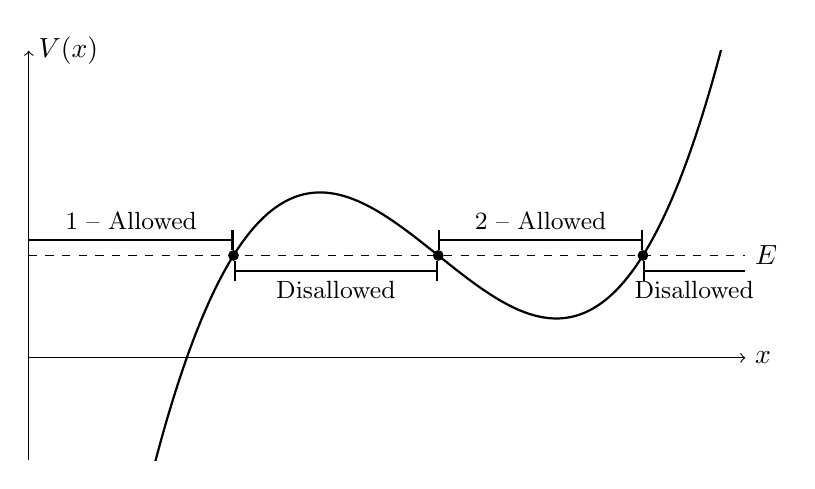
\begin{tikzpicture}[scale=1.3]
  \draw[->] (0, -2) -- (0, 2) node[right] {$V(x)$};
  \draw[->] (0, -1) -- (7, -1) node[right] {$x$};
  \draw[dashed] (0, 0) -- (7, 0) node[right] {$E$};


  \draw[-|, thick] (0, 0.15) -- (2, 0.15) node[midway, above] {\small 1 -- Allowed};
  \draw[|-|, thick] (2, -0.15) -- (4, -0.15) node[midway, below] {\small Disallowed};
  \draw[|-|, thick] (4, 0.15) -- (6, 0.15) node[midway, above] {\small 2 -- Allowed};
  \draw[|-, thick] (6, -0.15) -- (7, -0.15) node[midway, below] {\small Disallowed};

  \fill (2, 0) circle (1.5pt);
  \fill (4, 0) circle (1.5pt);
  \fill (6, 0) circle (1.5pt);

  \clip (0, -2) rectangle (7, 2);
  \draw[thick, domain=0:7, smooth, samples=100] plot (\x,{0.2*(\x - 2)*(\x - 4)*(\x - 6)});
\end{tikzpicture}
\end{center}
The points where $V(x) = E$ have $\dot{x} = 0$ and are called \textit{turning points}.
Typically, particles ``bounce off'' the potential at turning points and turn around.

Region 2 of the above graph is bounded so the particle bounces back and forth between turning points so its motion is bounded.
However, region 1 of the above graph is unbounded so the particle bounces off the turning point and then flies off to $x \to -\infty$ so its motion is unbounded.

A special cases occurs when $E = V(x_0)$ and $V'(x_0) = 0$:
\begin{center}
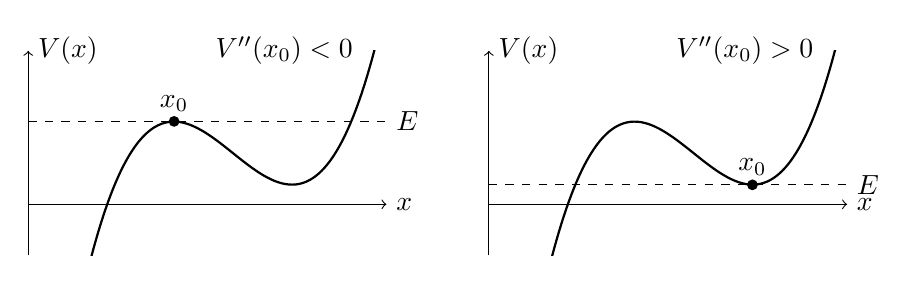
\begin{tikzpicture}[scale=1.3]
  \begin{scope}[scale=0.5]
    \node at (5, 2) {$V''(x_0) < 0$};
    \draw[->] (0, -2) -- (0, 2) node[right] {$V(x)$};
    \draw[->] (0, -1) -- (7, -1) node[right] {$x$};
    \draw[dashed] (0, 0.62) -- (7, 0.62) node[right] {$E$};
    \fill (2.85, 0.62) circle (3pt) node[above] {$x_0$};

    \clip (0, -2) rectangle (7, 2);
    \draw[thick, domain=0:7, smooth, samples=100] plot (\x,{0.2*(\x - 2)*(\x - 4)*(\x - 6)});
  \end{scope}

  \begin{scope}[scale=0.5, xshift=9cm]
    \node at (5, 2) {$V''(x_0) > 0$};
    \draw[->] (0, -2) -- (0, 2) node[right] {$V(x)$};
    \draw[->] (0, -1) -- (7, -1) node[right] {$x$};
    \draw[dashed] (0, -0.62) -- (7, -0.62) node[right] {$E$};
    \fill (5.15, -0.62) circle (3pt) node[above] {$x_0$};

    \clip (0, -2) rectangle (7, 2);
    \draw[thick, domain=0:7, smooth, samples=100] plot (\x,{0.2*(\x - 2)*(\x - 4)*(\x - 6)});
  \end{scope}
\end{tikzpicture}
\end{center}
Such $x_0$ are called \textit{equilibrium points}.
Particles with energy $E$ will sit there indefinitely as at these points:
\begin{align*}
  m\ddot{x} &= -V'(x_0) = 0 \implies \ddot{x} = 0 \\
  \frac{1}{2}m\dot{x}^2 &= V(x_0) - E = 0 \implies \dot{x} = 0
\end{align*}
So since $\dot{x} = \ddot{x} = 0$ at $x_0$, a particle of energy $E$ at $x_0$ stays at $x_0$.
\subsubsection{Motion Close to Equilibrium Points}
Motion close to an equilibrium point is especially simple.
We can Taylor expand about $x \approx x_0$ as follows:
\begin{align*}
  V(x) &= V(x_0) + (x - x_0)\underbrace{V'(x_0)}_{=0} + \frac{1}{2}(x - x_0)^2 V''(x_0) + \cdots \\
       &\approx V(x_0) + \frac{1}{2}(x - x_0)^2 V''(x_0)
\end{align*}
There are then three main cases:
\begin{proofcases}
  \begin{case}{$V''(x_0) > 0$}
    If $V''(x_0) > 0$ (i.e. a minimum point of $V$), then $V$ is approximately the potential for a harmonic oscillator:
    \begin{align*}
      m\ddot{x} &= - V'(x) \approx -(x - x_0)V''(x_0) \\
      \ddot{x} + \frac{V''(x_0)}{m}x &= x_0 V''(x_0) \\
      \implies x &= x_0 + A\cos(\omega t + \phi)
    \end{align*}
    which are oscillations with frequency $\omega = \sqrt{\frac{V''(x_0)}{m}}$.
    For small $A$, the amplitude is small so we stay close to the equilibrium point and so neglecting higher order terms in the Taylor expansion remains valid.
    This is called a \textit{stable equilibrium point}.
  \end{case}
  \begin{case}{$V''(x_0) < 0$}
    If $V''(x_0) < 0$ (i.e. a maximum point of $V$), then we get an \textit{unstable equilibrium point} and the solution looks like:
    \[
      x = x_0 + \widetilde{A}e^{\gamma t} + \widetilde{B}e^{-\gamma t}
    \]
    where $\gamma = \sqrt{\frac{-V''(x_0)}{m}}$.

    If $\widetilde{A} \neq 0$, then we have exponential growth so the particle moves far away from the equilibrium point rapidly and so the Taylor expansion breaks down quickly.
    The size of $\gamma$ tells us how quickly the particle moves away from the equilibrium point.

    If $\widetilde{A} = 0$ and $\widetilde{B} \neq 0$, then this corresponds to ``rolling'' up the potential with just enough energy to reach the top as $t \to \infty$.
    We can see this as when $t \to \infty$, $x \to x_0$ which is at the maximum.
  \end{case}
  \begin{case}{$V''(x_0) = 0$}
    If $V''(x_0) = 0$, then we would need to Taylor expand to a higher order to analyse the system.
  \end{case}
\end{proofcases}
\section{Dimensional Analysis}
\textit{Dimensional Analysis} is a way to get information about solutions to equations without having to solve them.
At a mathematical level, dimensional analysis the ability to rescale variables to remove certain constants from the equations.
\begin{example}[Period of a Pendulum]
  \label{pendulumDimensions}
  Later in this course we will derive the equation for a pendulum of length $\ell$:
  \[
    \deriv[2]{\theta}{t} = - \frac{g}{\ell}\sin \theta
  \]
  Suppose we release it from rest at some angle $\theta_0$ and want to know its period.
  That is, we wish to find the smallest positive $T$ such that $\theta(t + T) = \theta(t)\ \forall t$.

  We can remove $g$ and $\ell$ from the equation by rescaling $t = \sqrt{\frac{\ell}{g}} \tau$ and, for convenience, let $\theta(t(\tau)) = F(\tau)$.
  Using the chain rule we have:
  \[
    \deriv[2]{F}{\tau} = -\sin F
  \]
  This equation does not depend on $g$ and $\ell$ so neither can $F$.
  Because of this, the period $\Delta \tau$ of $F(\tau)$ may depend on the initial condition $\theta_0$ but cannot depend $g$ or $\ell$.
  \begin{align*}
    F(\tau + \Delta \tau) = F(\tau) \implies \theta(t) &= F\left(\sqrt{\frac{g}{\ell}}t\right) = F\left(\sqrt{\frac{g}{\ell}}t + \Delta \tau\right) \\
                                                       &= F\left(\sqrt{\frac{g}{\ell}}\left[t + \sqrt{\frac{\ell}{g}}\Delta \tau\right]\right) \\
                                                       &= \theta\left(t + \sqrt{\frac{\ell}{g}} \Delta \tau\right)
  \end{align*}
  So the period is $T = \sqrt{\frac{\ell}{g}} \Delta \tau$.
  Since we know that $\Delta \tau$ cannot depend on $\ell$ or $g$, this means that $T \propto \sqrt{\frac{\ell}{g}}$.
  So, without solving the equation, we learnt that the period of a pendulum is proportional to $\sqrt{\frac{\ell}{g}}$.
\end{example}
In general, the necessary rescaling may not be obvious.
We associate \textit{dimensions} to all constants and variables so that we do not have to manually carry out the rescaling process each time.
\begin{definition}[Basic Dimensions]
  The three basic dimensions are:
  \begin{itemize}
    \item \textit{Length} $L$
    \item \textit{Time} $T$
    \item \textit{Mass} $M$
  \end{itemize}
\end{definition}
\begin{remark}[Notation]
  We use the notation $[x]$ to mean the dimensions of $x$.
\end{remark}
\begin{example}
  \begin{enumerate}
    \item $[\dot{x}] = LT^{-1}$, $[\ddot{x}] = LT^{-2}$ as they are derivatives of a length with respect to a time.
    \item $F = m\ddot{x}$ so $[F] = MLT^{-2}$.
    \item $E = \frac{1}{2}m\dot{x}^2$ so $[E] = ML^2T^{-2}$.
  \end{enumerate}
\end{example}
It is sometimes useful to introduce additional dimension such as charge or temperature depending on the problem but length, time, and mass are usually sufficient.
All arguments of non-trivial functions, that is, functions involving sums of different powers, must be dimensionless as we cannot sum quantities of different dimensions.
For example, if we are taking $\sin \theta$, we must have $[\theta] = 1$.

The fundamental rule of dimensional analysis is that for all equations, the dimensions on the right hand side and left hand side must be consistent.
\begin{example}[Pendulum Revisited]
  We first find the dimensions of all of the data (i.e. constants and variables) involved:
  \[
    [g] = LT^{-2},\ [\ell] = L,\ [m] = M,\ [\theta_0] = 1
  \]
  Note that we know that $\theta_0$ is dimensionless as it is the argument to a $\sin$ function.
  We want $[T] = T$.
  The choice of $T$ as a variable name here is a little confusing, we want the quantity $T$ to have dimensions of time.

  $T$ can only depend on data that we have so must be in the form $T = f(\theta_0)g^{A}\ell^{B}M^{C}$ for constants $A, B, C, D$.
  We use $f(\theta_0)$ since $\theta_0$ is dimensionless so any $f(\theta_0)$ is also dimensionless.

  For the dimensions to be consistent we require:
  \[
    T = [T] = [g]^{A}[\ell]^{B}[m]^{C} = L^{A}T^{-2A}L^{B}M^{C}
  \]
  Therefore, we must have $C = 0$, $A = -\frac{1}{2}$, $B = \frac{1}{2}$ so:
  \[
    T = f(\theta_0) \sqrt{\frac{\ell}{g}} \implies T \propto \sqrt{\frac{\ell}{g}}
  \]
  which is consistent with our result from \cref{pendulumDimensions}.
\end{example}
\begin{remark}[Note]
  When writing the form of the solution, we must include a function of any possible dimensionless combinations.
  In the above example, the only dimensionless combination was $\theta_0$.
  However, if the powers are not uniquely fixed by this process, we end up with dimensionless combinations of multiple constants and so we must include a function of any such combinations when formulating the trial solution.

  See Q7 on Example Sheet 1 for an example of this.
\end{remark}
\section{Friction}
\label{frictionDrag}
\begin{remark}[Note]
  In this section of the course, we will cover \textit{fluid drag} (friction due to an object moving through a fluid), however later in the course (\cref{dryFriction}), we will study \textit{dry friction} (friction between two objects in contact with each other).
\end{remark}
When objects move from a medium (e.g. air or water) there are \textit{microscopic} forces between the object and the medium.
These forces cause the momentum of the object to be carried off into the medium and lost.

\textit{Friction} is a \textit{macroscopic} force that keeps track of the momentum lost due to the complicated microscopic effects.

Friction has two important properties:
\begin{enumerate}
  \item Friction \textbf{does not conserve the energy} of the object as energy is lost to the medium.
    This energy is lost as \textit{heat}.
  \item Friction is \textbf{irreversible}.
    That is, energy is lost by the object and never gained.
    If you are ever in doubt about the sign of a friction force, it should always act in the opposite direction to velocity, in order to slow the object down.
\end{enumerate}
\subsection{Fluid Drag}
There are two important cases of fluid drag.
\begin{definition}[Linear Drag]
  Linear drag is drag proportional to the speed of the object:
  \[
    \vec{F} = -k_1 \vec{v}
  \]
  for a \textit{coefficient of friction} $k_1$.
\end{definition}
Linear drag depends on \textit{viscous effects} (see IB Fluid Dynamics).
This is when the object moves the medium close to the object along with it.

Stokes' Law for a spherical object for radius $L$ tells us that:
\[
  k_1 = 6\pi \eta L
\]
where $\eta$ is the \textit{viscosity} of the fluid.
\begin{definition}[Quadratic Drag]
  Quadratic drag is drag proportional to the square of the speed of the object:
  \[
    \vec{F} = -k_2 |\vec{v}|\vec{v}
  \]
  for a \textit{coefficient of friction} $k_2$.
  Note that we use the absolute value to ensure that always acts in the opposite direction to the velocity.
\end{definition}
Quadratic drag is the more intuitive of these two cases.
The object bumps into molecules at a rate proportional to its velocity and the change in momentum per collision is also proportional to velocity, so it is reasonable to expect the drag to be proportional to the square of the velocity.

The number of collisions should be proportional to the density of the medium $\rho$ and the cross-sectional area $A$, so we might expect that $k_2 \propto \rho A$.
We can check the units of this using dimensional analysis:
\[
  [F] = MLT^{-2},\ [k_2 v^2] = ML^{-3}L^2L^2T^{-2} = MLT^{-2}
\]
which is consistent, so any other factors must be dimensionless.

Both linear and quadratic drag are typically present, however, which one dominates depends on the \textit{Reynold's Number} $R$:
\[
  \frac{F_{\text{quad}}}{F_{\text{lin}}} \sim \frac{\rho A v^2}{\eta L v} \sim \frac{\rho L v}{\eta} = R
\]
This tells us the relative importance of quadratic and linear drag and will be covered further in IB Fluid Dynamics.
\begin{remark}
  $x$ and $\ddot{x}$ are invariant under a \textit{time reversal} $t \mapsto -t$, however, $\dot{x}$ is not.

  As far as we know, the fundamental laws of nature are all invariant under \textit{CPT} (Charge reversal $q \mapsto -q$, Parity reversal $x \mapsto -x$, and Time reversal $t \mapsto -t$).

  As $\dot{x}$ is not invariant under time reversal, friction forces are not invariant under time reversals and therefore they cannot be fundamental forces.
\end{remark}
\subsection{Terminal Velocity}
Consider an object falling with quadratic friction under gravity:
\begin{equation}
  m \deriv{v}{t} = - mg + kv^2 \label{termDE}
\end{equation}
\begin{remark}[Note]
  Here we are considering motion in one dimension, however, as we have seen, we can also have motion (and therefore friction) in different directions to gravity.
  We can model such situations using a vector differential equation:
  \[
    m \dot{\vec{v}} = m\vec{g} - k|\vec{v}|\vec{v}
  \]
\end{remark}
\subsubsection{Analysis Without Solving}
We know that the friction needs to act in the opposite direction to the velocity.
The object is falling downwards so we need the friction to act upwards, and hence it needs to have the opposite sign to $g$.

If the object starts at rest, the initial acceleration of the object is exactly $-g$.
As the velocity of the object increases, so does the magnitude of the drag force, so the downwards force, and therefore the acceleration, on the object decreases.
As this continues, the downwards force asymptotically approaches 0, and so the acceleration approaches 0.
This means that the velocity must approach a constant value.
This is called the \textit{terminal velocity} of the object.

Since we need the acceleration to be 0, we must have $kv^2_{\text{term}} = mg$ and so:
\[
  v_{\text{term}} = - \sqrt{\frac{mg}{k}}
\]
Unlike the escape velocity (see \cref{escapeVelocity}), this is dependant on mass.
This means that heavier objects reach a greater terminal velocity than lighter ones.
For a raindrop, $v_{\text{term}} \approx \qty{10}{\metre\second^{-1}}$.

\subsubsection{Solving Directly}
\Cref{termDE} is separable so we can solve for $t$ as a function of $v$ yielding:
\begin{equation}
  t = -\sqrt{\frac{m}{kg}}\artanh\left(\sqrt{\frac{k}{mg}}v\right) \label{eqnDragT}
\end{equation}
Rearranging for $v$, we have:
\[
  v = -\sqrt{\frac{mg}{k}}\tanh\left(\sqrt{\frac{kg}{m}}t\right)
\]
As $t \to \infty$, $\tanh\left(\sqrt{\frac{kg}{m}}t\right) \to 1$ and so $v \to -\sqrt{\frac{mg}{k}} = v_{\text{term}}$.
\subsubsection{Approximate Timescale}
We can use dimensional analysis to approximate the timescale with which the object reaches its terminal velocity.
To find the units for $k$, we know that both terms of the right hand side of \cref{termDE} must be dimensionally consistent so:
\[
  [k][v]^2 = [m][g] \implies [k]L^2T^{-2} = MLT^{-2} \implies [k] = ML^{-1}
\]
The approximate timescale for it to reach terminal velocity can only depend on $m$, $g$ and $k$ so:
\begin{align*}
  t_0 &\propto m^{A}g^{B}k^{C} \\
  \implies T &= M^{A}L^{B}T^{-2B}M^{C}L^{-C}
\end{align*}
So we must have $A = \frac{1}{2}$, $B = -\frac{1}{2}$, and $C = -\frac{1}{2}$.
Therefore:
\[
  t_0 \propto \sqrt{\frac{m}{kg}}
\]
\begin{remark}
  Since the terminal velocity is approached asymptotically, the velocity never actually reaches $v_0$ so $t_0$ is not ``the time to reach terminal velocity''.

  We can however ask how long it takes for the object to get to some proportion $p$ of the terminal velocity.
  If we substitute $-p \sqrt{\frac{mg}{k}}$ into \cref{eqnDragT}, we then have:
  \[
   t_0 = \sqrt{\frac{m}{kg}}\artanh(p) \implies t_0 \propto \sqrt{\frac{m}{kg}}
  \]
  which agrees with our result using dimensional analysis as $\tanh(p)$ must be dimensionless.
\end{remark}
\subsection{Damping}
Drag also \textit{damps} the small oscillations about a stable equilibrium point.
For small oscillations, typically linear drag is more important so we can approximate this as the damped harmonic oscillator:
\[
  \ddot{x} = -\omega^2_0 x - 2\alpha \dot{x}
\]
where $\omega_0$ is the angular frequency and $\alpha$ is a coefficient of friction.
\[
  x = e^{-\alpha t} (A_+ e^{i \Omega t} + A_- e^{-i\Omega t})
\]
where $\Omega = \sqrt{\omega^2_0 - \alpha^2}$ and we take the real part of $x$.
There are three cases:
\begin{proofcases}
  \begin{case}{$\omega^2_0 > \alpha^2$ -- Underdamping}
    This leads to decaying oscillations as $\Omega$ is real.
  \end{case}
  \begin{case}{$\omega^2_0 < \alpha^2$ -- Overdamping}
    This leads to exponential decay back to equilibrium as $\Omega$ is imaginary.
  \end{case}
  \begin{case}{$\omega^2_0 = \alpha^2$ -- Critical Damping}
    In this case, we get decay of form $x = (A + t)e^{-\alpha t}$ as $\Omega = 0$.
  \end{case}
\end{proofcases}
We solved this in IA Differential Equations and it is discussed in further detail there.
\end{document}
